% 
% Annual CCN conference
% Sample LaTeX Two-Page Summary -- Proceedings Format
% based on the prior cognitive science style file

% Original : Ashwin Ram (ashwin@cc.gatech.edu)       04/01/1994
% Modified : Johanna Moore (jmoore@cs.pitt.edu)      03/17/1995
% Modified : David Noelle (noelle@ucsd.edu)          03/15/1996
% Modified : Pat Langley (langley@cs.stanford.edu)   01/26/1997
% Latex2e corrections by Ramin Charles Nakisa        01/28/1997 
% Modified : Tina Eliassi-Rad (eliassi@cs.wisc.edu)  01/31/1998
% Modified : Trisha Yannuzzi (trisha@ircs.upenn.edu) 12/28/1999 (in process)
% Modified : Mary Ellen Foster (M.E.Foster@ed.ac.uk) 12/11/2000
% Modified : Ken Forbus                              01/23/2004
% Modified : Eli M. Silk (esilk@pitt.edu)            05/24/2005
% Modified : Niels Taatgen (taatgen@cmu.edu)        10/24/2006
% Modified : David Noelle (dnoelle@ucmerced.edu)     11/19/2014
% Modified : Konrad Kording (koerding@gmail.com) 2/15/2017

\documentclass[10pt,letterpaper]{article}

\usepackage{ccn}
\usepackage{pslatex}
\usepackage{apacite}
\usepackage{graphicx}


\graphicspath{ {../static/} }

\title{Convolutional neural networks performing a visual search task show attention-like 
limits on accuracy when trained to generalize across multiple search stimuli}
 
\author{{\large \bf David A. Nicholson (dnicho4@emory.edu)} \\
  \AND {\large \bf Astrid A. Prinz (astrid.prinz@emory.edu)} \\
  Emory University Department Of Biology, 1510 Clifton Road, Atlanta, GA 30322}


\begin{document}

\maketitle

\section{Abstract}
{
\bf
What limits our ability to find what we are looking for in the cluttered noisy world? To investigate this, cognitive scientists have long used visual search. In spite of hundreds of studies, it remains unclear how to relate effects found using the discrete item display search task to computations in the visual system. A separate thread of research has studied the visual system of humans and other primates using convolutional neural networks (CNNs) as models. Multiple lines of evidence suggest that training CNNs to perform tasks such as image classification causes them to learn  representations similar to those used by the visual system. These studies raise the question of whether CNNs that have learned such representations behave similarly to humans performing other vision-based tasks. Here we address this by measuring the behavior of CNNs trained for image classification while they perform the discrete item display search task. We first show how a fine-tuning approach often used to adapt pre-trained CNNs to new tasks can produce models that show human-like limitations on this task. However we then demonstrate that we can greatly reduce these effects by changing training,without changing the learned representations. Lastly we show that accuracy is not impaired when single networks are trained to discriminate multiple types of visual search stimuli. Based on these findings, we suggest that CNNs are not necessarily subject to the same limitations as the primate visual system.
}
\begin{quote}
\small
\textbf{Keywords:} 
attention;visual search
\end{quote}

\section{Introduction}

\begin{figure}[!ht]
\begin{center}
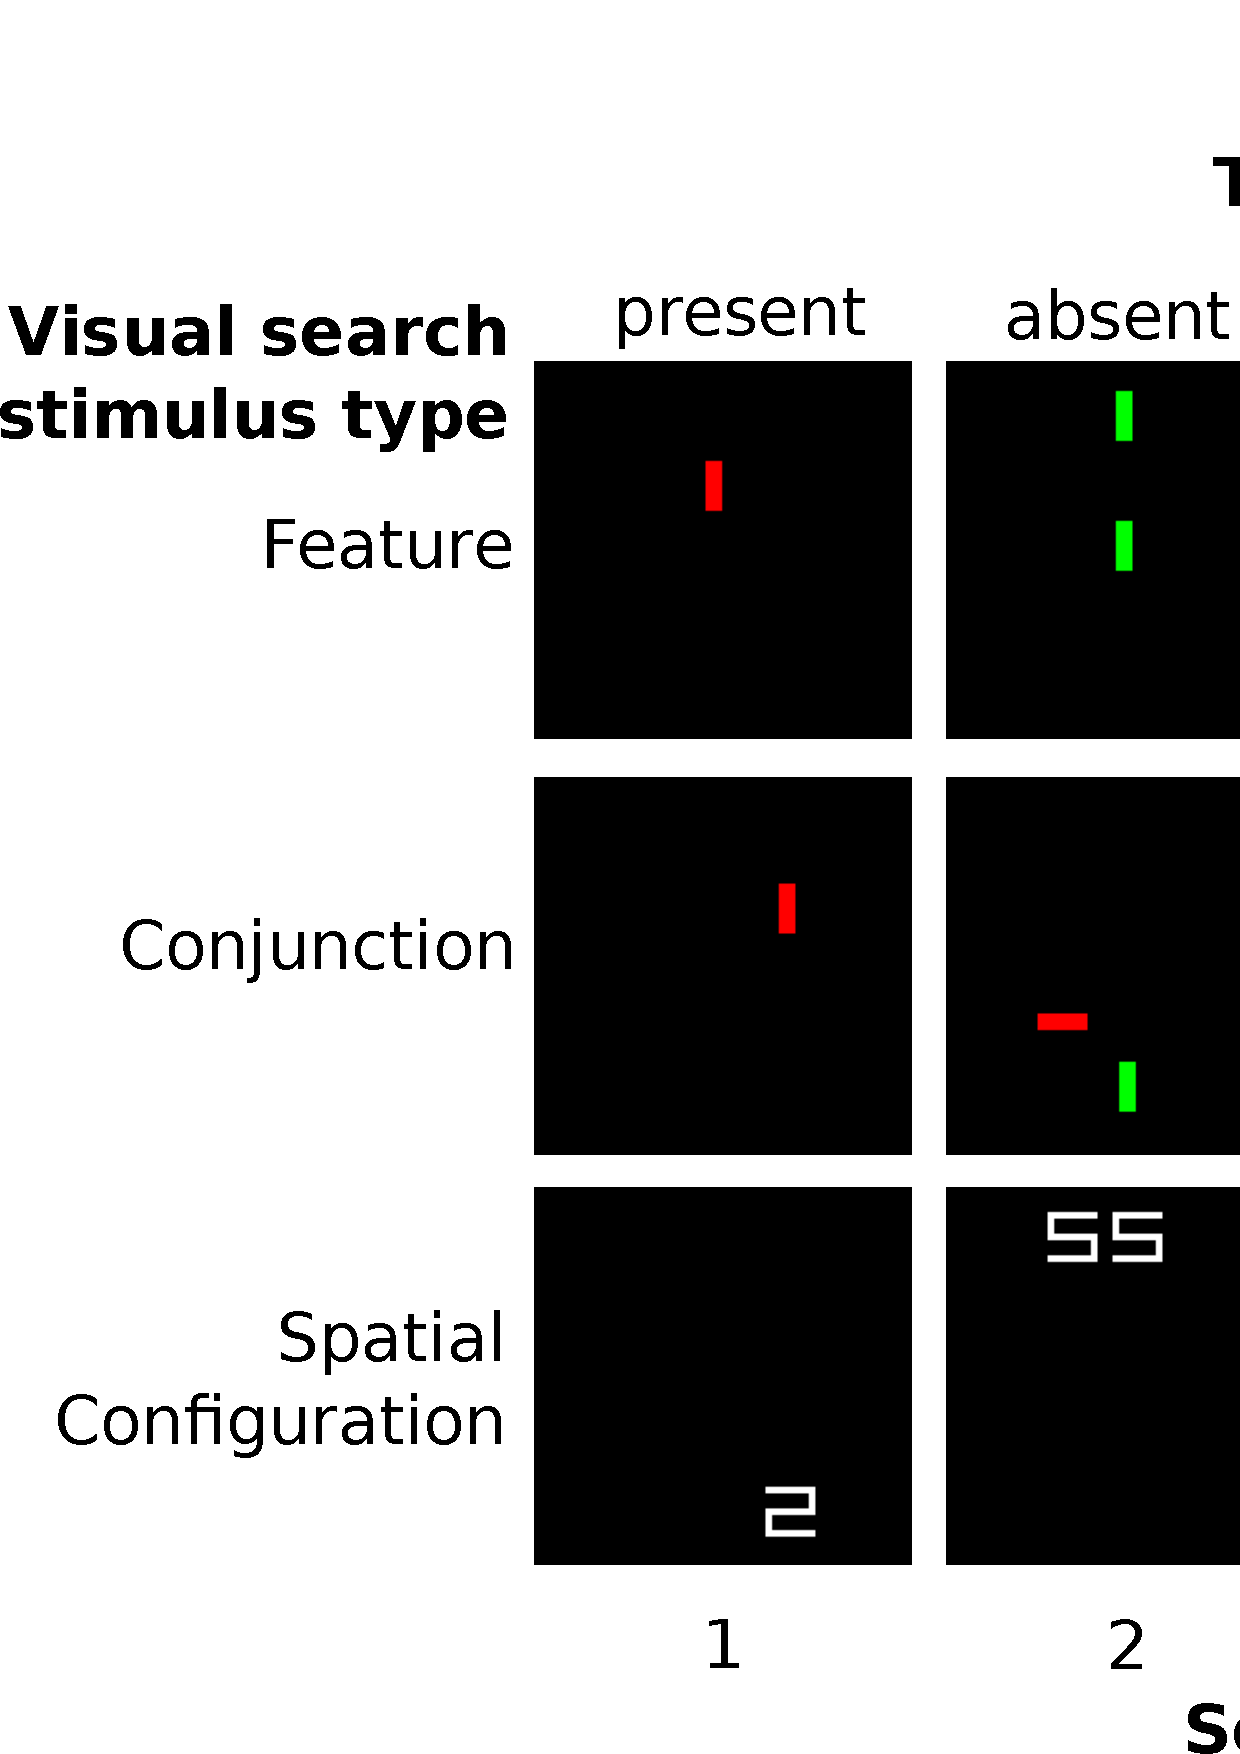
\includegraphics[width=\columnwidth]{fig1/fig1.png}
\end{center}
\caption{
\textbf{The discrete item display search task}. On each trial, subjects view  
 a display (example images, \textbf{a}) of discrete items on a flat background. Subjects 
respond whether the target is present or absent (condition varies across rows 
of \textbf{a}). Another condition that varies across trials is the set size, that is, 
the total number of targets and distractors (varies across rows in \textbf{a}). Many studies 
focus on set size effects. Typical effects are an increase in reaction time 
or a decrease in accuracy as set size increases (depicted schematically in \textbf{b}, 
redrawn from \cite{wolfeReactionTimeDistributions2010} and \cite{ecksteinLowerVisualSearch1998a}). 
Effects vary based on the features that distinguish targets from distractors 
(shown in columns). Details in introduction. Accuracy for spatial configuration-type 
stimuli not shown in \textbf{b} because this has been less studied (but see 
\cite{palmerSignalDetectionEvidence2011}).
}
\label{fig1}
\end{figure}

What limits our ability to find what we are looking for in the cluttered noisy world we 
see around us? One of the principle tasks that has been used to investigate this question 
is a visual search task (Figure~\ref{fig1}) \cite{wolfeVisualSearch1998}
we will refer to as the \emph{discrete item display search} task. 
Most studies using this task experimentally manipulate factors such as features of the targets and 
distractors in order to identify those factors that limit visual search 
\cite{ecksteinVisualSearchRetrospective2011,wolfeFiveFactorsThat2017}, known as 
\emph{capacity limitations}. There are essentially two models of capacity limitations: 
\emph{attention-limited} and \emph{noise-limited} models \cite{palmerSignalDetectionEvidence2011}. 
Briefly, we review these and describe how they depend in part on the 
way the visual search task is performed. Both models 
depend on what are known as \emph{set-size effects} seen when using visual search stimuli, 
depicted schematically in \ref{fig1}\textbf{b}).
Attention-limited models posit two-stage theories of visual processing, a first 
\emph{preattentive} stage which can process single features such as color or orientation 
in parallel, and a second \emph{attentive} stage which requires a serial computation to 
binds features, resulting in a bottleneck 
\cite{treismanFeatureintegrationTheoryAttention1980,wolfeGuidedSearchAlternative1989,wolfeGuidedSearchRevised1994}. 
Evidence for this theory came from visual search 
experiments where subjects were shown stimuli until responding, and their reaction time 
was measured. Plotting reaction time as a function of set size revealed 
lines whose slope were near zero (\ref{fig1}\textbf{b}, top row, left plot) 
when a single feature distinguished the target from 
distractors (\ref{fig1}, \textbf{a}, left column). 
The slope of reaction time versus set size increased though (\ref{fig1}\textbf{b}, top row, middle plot), 
when distinguishing the target from distractors required finding a 
conjunction of features (\ref{fig1}\textbf{a}, middle column). Slopes became 
even steeper (\ref{fig1}\textbf{b}, top row, right plot) 
when targets and distractors shared features and could only be 
distinguished by their spatial configuration (\ref{fig1}\textbf{a}, right column). 
This sort of set size effect has been replicated hundreds of times, although it remains 
unclear why some search stimuli are processed effectively in parallel while others 
face a bottleneck \cite{wolfeWhatCanMillion1998,wolfeFiveFactorsThat2017}.
The second family of capacity limitations conceives of visual search as completely parallel but 
noisy. These models arose in large part in reaction 
to the way the visual search task was carried out when investigating
serial mechanisms. Early studies that measured reaction times left several factors 
uncontrolled, such as target-distractor similarity \cite{duncanVisualSearchStimulus1989}, 
drops in acuity outside the fovea, eye movements, and effects resulting from visual 
crowding \cite{ecksteinLowerVisualSearch1998a}. 
Hence researchers designed versions of the visual search task that controlled for such 
factors. Crucially, they showed subjects the 
stimulus only briefly, to prevent eye movements, and measured accuracy instead of reaction
time (shown schematically in \ref{fig1}\textbf{b}, bottom row). 
Computational models of parallel mechanisms, based on signal detection theory, 
successfully explained results from feature and conjunction search stimuli 
(\ref{fig1}\textbf{a}, left and middle columns) 
\cite{palmerPsychophysicsVisualSearch2000,ecksteinVisualSearchRetrospective2011}.

In spite of nearly half a century of studies based on the discrete item display search task,
this core question remains unresolved: to what extent can limitations be attributed to an attention-like 
computation, e.g. binding features into items, and to what extent can those limitations be 
attributed to other computations, e.g. a decision-making process subject to noisy internal representations?
To foreshadow our approach, we suggest another way of posing this question: 
if some algorithm could produce a statistical model capable of learning from data 
to classify visual search stimuli as target present or absent with high 
accuracy, would that accuracy still be subject to some ceiling, due simply to the 
constraints of the task? This framing bears some similarity to a 
well-established framework in vision research known as ideal observer analysis 
\cite{geislerIdealObserverAnalysis2003}. However, few ideal observer models have taken the 
form of "pixel-in, behavior-out", and therefore do not generalize to many 
different types of visual search stimuli, so their predictive power is limited 
\cite{geislerModelsOvertAttention2011}.

Both attention-limited and noise-limited models are highly abstracted models of the visual system,
in which low-level features pass through a hierarchy until reaching a final stage consisting of
a simple decision rule.
Similarly, the architecture of convolutional neural networks (CNNs) now routinely used for
computer vision tasks represents a highly abstracted view of the visual system.
Many researchers have drawn parallels between the architecture of CNNs and the 
architecture of the visual system in the brain \cite{kriegeskorteDeepNeuralNetworks2015}, 
in particular in humans and other primates where this system has been most thoroughly 
studied. Like CNNs, the visual system has a hierarchical structure, and is thought to 
function in part by performing transformations at each level of this hierarchy so that 
high-dimensional, low-level features are mapped into low-dimensional abstract 
representations. Several recent studies have found that that, when optimized to perform 
tasks such as image classification, CNNs learn representations similar to those 
observed in the visual system
\cite{yaminsUsingGoaldrivenDeep2016, yaminsPerformanceoptimizedHierarchicalModels2014}. 
These studies raise the question of whether CNNs that have learned such 
representations behave similarly to humans performing other vision-based tasks. 
Here we address this by measuring the behavior of CNNs trained for image classification 
while they perform the discrete item display search task.
While there have been previous studies of neural networks 
performing visual search tasks, we are aware of only one study \cite{poderCapacityLimitationsVisual2017} 
that employed the sort of CNN architectures used in studies of the visual system referenced above.
We replicate the methods from that study, and extend that author's results.
In the interest of replicability, we have made the code and summary results \footnote{https://github.com/NickleDave/visual-search-nets} 
available, and will release the raw data upon publication \footnote{at https://figshare.com/articles/visual-search-nets/7688840}.

\section{Results}

\begin{figure}[!ht]
\begin{center}
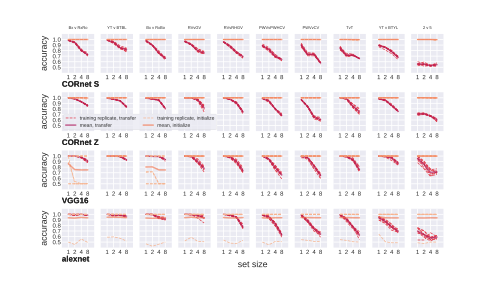
\includegraphics[width=\columnwidth]{fig2/fig2.png}
\end{center}
\caption{
\textbf{Human-like limits on accuracy of CNNs performing the discrete item display search task}
As described in the text, when using weights pre-trained on ImageNet in convolutional layers, 
and fine-tuning weights in fully-connected layers so AlexNet could perform the task, 
this CNN showed decreases in accuracy as set size increased (\textbf{a}). This decrease was 
smallest for feature search stimuli (left plot), intermediate for conjunction stimuli (middle plot), 
and largest for spatial configuration stimuli (right plot). The same approach produced similar 
results with the VGG16 architecture (\textbf{b}).
} 
\label{fig2}
\end{figure}

As referenced above, previous work suggests that optimizing CNNs to perform image 
classification causes them to acquire representations which resemble those that can 
be identified in the brain. We first tested whether the CNN architecture AlexNet 
\cite{krizhevskyImagenetClassificationDeep2012}
would be subject to human-like limits on the discrete item display search task, 
when utilizing representations learned by optimizing the weights for image classification 
on the ImageNet dataset \cite{dengImagenetLargescaleHierarchical2009}. 
To do so, we used a \emph{fine-tuning} approach, in which we used pre-trained weights in earlier 
convolutional layers of AlexNet, but randomly initialized weights in the later 
fully-connected layers \cite{yosinskiHowTransferableAre2014}.
More specifically, we replicated the training method described in
\cite{poderCapacityLimitationsVisual2017}, where we trained each network that we tested with 
6400 samples of \emph{one} of the visual search stimuli (e.g. feature search), and then 
measured accuracy on a separate test set of 800 samples. Stimuli were generated with a 
small Python package \footnote{https://github.com/NickleDave/searchstims} 
which produced images the same size as the images used to train on 
ImageNet, and were pre-processed in the same way as those images, 
except that no re-sizing was done.
This training method produced AlexNet models whose accuracy showed set-size dependence 
similar to human subjects (Figure \ref{fig2}\textbf{a}). 
For the three types of visual search stimuli that we used, there was a set size effect,
where accuracy decreased as the set size increased. 
This effect was smallest for feature search (left column), slightly 
larger for conjunction search (middle column), and largest for spatial configuration 
search. To test whether this effect was unique to AlexNet, we also used the same approach 
with the VGG16 architecture, and produced similar results (Figure \ref{fig2}\textbf{b}). 
In addition to finding set size effects that were qualitatively 
similar to those seen in human subjects, we also noted that accuracy was always higher 
for the "target absent" condition. We do not find reports of similar differences between 
target present and target absent conditions in human subjects.

\begin{figure}[ht]
\begin{center}
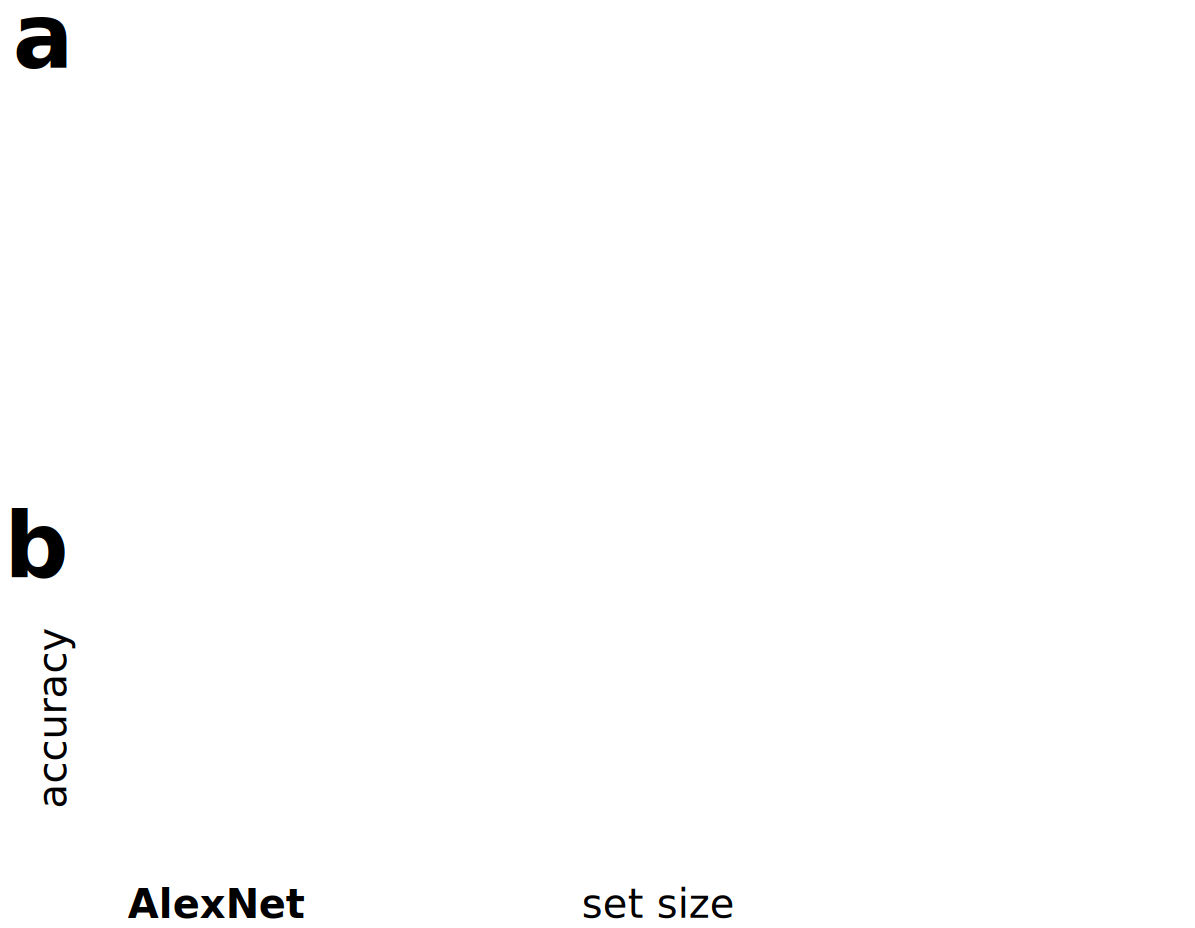
\includegraphics[width=\columnwidth]{fig3/fig3.png}
\end{center}
\caption{
\textbf{Changing training greatly reduces set size effects.}
Training histories showed that the accuracy of models trained 
with the fine tuning approach did not converge
on some asymptotic value, and 
varied depending on the set size of the search stimuli (\textbf{a}, left plot). 
Increasing the learning rate and including more examples of stimuli with 
larger set sizes greatly sped up convergence (\textbf{a}, right plot).
AlexNet models trained with this higher learning rate and larger training set
showed reduced set size effects (\textbf{b}).
} 
\label{fig3}
\end{figure}

Because accuracy of CNNs depends in part on training, it could be the case that 
the results just described are an artifact of how we trained the networks. 
To gain insight into how our results depended on training, 
we plotted training histories where we measured accuracy on the training set 
at each epoch \emph{separately for each set size in the visual search stimuli}.
These plots revealed (1) that accuracy had not yet approached some asymptotic 
value by the end of training, and (2) that there was an inverse relationship between 
the set size of a visual search stimulus and the rate that its accuracy increased, 
e.g. accuracy on set size 1 reached its highest value within a few epochs, while accuracy on 
set size 8 never converged on an asymptotic value (figure \ref{fig3}\textbf{a}).
Because these plots showed accuracy had not converged when we stopped training, we 
used random search to find an optimal learning rate, a key hyperparameter.
We did find we were able to improve accuracy and decrease training time by 
using a typical learning rate on the fully-connected layers, while simply 
freezing the pre-trained weights in earlier convolutional layers.
Based on the the observation that different set sizes converged at different rates, we 
also augmented the number of samples for larger set sizes.
It may seem counterintuitive to "unbalance" the dataset this way, until one considers 
that there are many more combinations of displays of set size 8 then of set size 1. 
For example, if items are located on a 5-by-5 grid, then for set size 1 there are 25-pick-1
combinations, i.e. 25,  while for set size 8 there are 25-pick-8 combinations (approximately 100k).
(Note that the library we used to generate images ensures that there are no repeats; for set size 1, 
jitter is added to produce more than 25 possible displays; this is typically done in experiments 
with human subjects, and acts as a form of data augmentation for neural networks.)
We simply multiplied the number of samples by the set size, since scaling 
by the number of possible combinations would have produced prohibitively large datasets.
After making these changes to the learning rate and the statistics of the dataset, 
we saw that the set size effects were greatly reduced \ref{fig3}\textbf{b}. This indicates 
that these effects are due in least at part to how we trained the networks.

Because neural networks, including CNNs, act as function approximators, it could also be the case 
that they were able to perform the discrete item display search task with relatively high 
accuracy simply by learning an exclusive-or function for the single search stimulus that we trained 
them to classify. A more rigorous test would be to train single networks to classify multiple 
stimuli, in the same way that humans do in discrete item display search experiments. 
As a final test, we trained two instances of Alexnet on very large datasets containing 
all three stimuli used in this study \ref{fig4}. We found similar accuracy as shown in \ref{fig3}, 
even when single networks were challenged to perform this task with multiple stimuli.

\begin{figure}[!ht]
\begin{center}
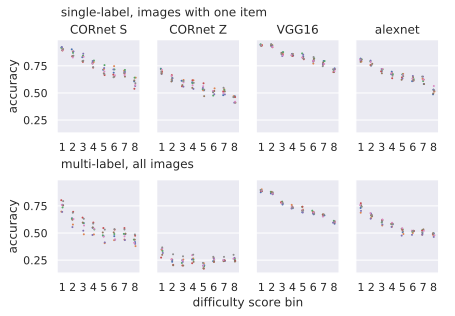
\includegraphics[width=\columnwidth]{fig4/fig4.png}
\end{center}
\caption{
\textbf{Training single networks on multiple stimuli does not impair accuracy}
Two instances of AlexNet trained on datasets containing all three types of visual search 
stimuli used in this study still attained high accuracy.
} 
\label{fig4}
\end{figure}

\section{Discussion}
We tested whether CNNs using representations learned from image classification tasks would be subject 
to human-like capacity limitations when performing the discrete item display search task. While we 
did not find that CNNs can always perform the discrete item display search task with perfect accuracy, 
we did show that these models are not necessarily limited by the same factors as the primate visual system.

\section{Acknowledgments}
Research funded by the Lifelong Learning Machines program, 
DARPA/Microsystems Technology Office, DARPA cooperative agreement HR0011-18-2-0019.
David Nicholson was partially supported by the 2017 William K. and Katherine W. Estes Fund
to F. Pestilli, R. Goldstone and L. Smith, Indiana University Bloomington.
Thank you to Zsolt Kira and Yen-Chang Hsu for feedback on results,
and for suggesting changes to training methods.
Thank you also to Constantine Dovrolis and Sarah Pallas for feedback on earlier versions 
of this work.

\bibliographystyle{apacite}

\setlength{\bibleftmargin}{.125in}
\setlength{\bibindent}{-\bibleftmargin}

\bibliography{ccneuro2019}


\end{document}
